% Copyright (c) 2013-2016 Christian Dietrich
%
% This work may be distributed and/or modified under the
% conditions of the LaTeX Project Public License, either version 1.3
% of this license or (at your option) any later version.
% The latest version of this license is in
%   http://www.latex-project.org/lppl.txt
% and version 1.3 or later is part of all distributions of LaTeX
% version 2005/12/01 or later.
%
% This work has the LPPL maintenance status `maintained'.
%
% The Current Maintainer of this work is Christian Dietrich
%
% This work consists of the files dataref.tex and dataref.sty

\documentclass{ltxdoc}
\usepackage[usagereport]{dataref}[2015/09/17]

\EnableCrossrefs
\CodelineIndex
\RecordChanges

\usepackage{verbatim}
\usepackage{listings}
\usepackage{pdfcomment}
\usepackage{siunitx}
\usepackage{xspace}
\usepackage{pgffor}
\usepackage{filecontents}
\usepackage{tikz}
\usetikzlibrary{positioning, arrows}

\begin{filecontents}{datapoints.tex}
\drefset{/control group/mice race}{Black Six}
\drefset{/control group/mice count}{32}
\drefset{/control group/dead after 24h}{4}
\drefset{/control group/dead after 48h}{7}
\drefset{/control group/recovered}{21}

\drefset{/med A/mice race}{Black Six}
\drefset{/med A/mice count}{32}
\drefset{/med A/dead after 24h}{6}
\drefset{/med A/dead after 48h}{12}
\drefset{/med A/recovered}{20}

\drefsethelp{.*/mice race}{The mice race used for experiments heavily
     influences the outcome of the results}

\drefsethelp{.*/(dead after|recovered)}{Of all infected mice, a
  certain number died within a specified period of time. A certain
  recovered from the infection. The dead categories are cumulative and
include all dead mice before.}
\end{filecontents}
\input{datapoints}
% \OnlyDescription
\drefkeys{prefix=/foo,value=123,save=/foo}
\drefset{/override test}{2}
\begin{document}
\drefsave{/override test}{4}
\drefkeys{prefix=}

\CheckSum{0}


 \CharacterTable
  {Upper-case    \A\B\C\D\E\F\G\H\I\J\K\L\M\N\O\P\Q\R\S\T\U\V\W\X\Y\Z
   Lower-case    \a\b\c\d\e\f\g\h\i\j\k\l\m\n\o\p\q\r\s\t\u\v\w\x\y\z
   Digits        \0\1\2\3\4\5\6\7\8\9
   Exclamation   \!     Double quote  \"     Hash (number) \#
   Dollar        \$     Percent       \%     Ampersand     \&
   Acute accent  \'     Left paren    \(     Right paren   \)
   Asterisk      \*     Plus          \+     Comma         \,
   Minus         \-     Point         \.     Solidus       \/
   Colon         \:     Semicolon     \;     Less than     \<
   Equals        \=     Greater than  \>     Question mark \?
   Commercial at \@     Left bracket  \[     Backslash     \\
   Right bracket \]     Circumflex    \^     Underscore    \_
   Grave accent  \`     Left brace    \{     Vertical bar  \|
   Right brace   \}     Tilde         \~}


 \changes{v0.4}{2015/04/21}{Remove Spurious Whitespaces}
 \changes{v0.1}{2013/12/06}{Initial version}

 \DoNotIndex{\newcommand,\newenvironment}

  \def\colorfirsttoken#1#2{\bgroup\expandafter\color{#1}\cmd{#2}\egroup}
\renewcommand{\meta}[1]{\bgroup\color{green!40!black}$\langle$\textit{#1}$\rangle$\egroup}
\newcommand{\Macro}[2][]{%
   \noindent\hspace{-\marginparwidth}%
   \mbox{\colorfirsttoken{blue!50!black}#2} \hfill\mbox{#1}\par}
 \newcommand{\Option}[2][]{%
   \noindent\hspace{-\marginparwidth}%
   \mbox{\color{red!50!black}#2} \hfill\mbox{#1}\par}

 \colorlet{examplefill}{yellow!80!black}
 \definecolor{codebackground}{rgb}{0.9,0.9,1}
 \newdimen\examplewidth
 \newsavebox{\codebox}
 \newenvironment{example}[1][\marginparwidth-12pt]
 {\begin{lrbox}{\codebox}\begin{minipage}{#1}}
 {\end{minipage}\end{lrbox}%
   \examplewidth=\wd\codebox%
   \addtolength{\examplewidth}{-1.2\marginparwidth}%
   \global\examplewidth=\examplewidth%
  \noindent\hspace{-0.8\marginparwidth}\colorbox{examplefill}{\usebox{\codebox}}\hspace{12pt}}

 \newenvironment{codeexample}
 {\begin{lrbox}{\codebox}\begin{minipage}{\textwidth+\examplewidth}}
{\end{minipage}\end{lrbox}\noindent\colorbox{codebackground}{\usebox{\codebox}}\global\examplewidth=0pt%
\par\vspace{1em}}%


 \newcommand{\dataref}{\textsc{dataref}\xspace}
 \providecommand*{\url}{\texttt}
 \GetFileInfo{dataref.sty}
 \title{The \textsf{dataref} package}
 \author{Christian Dietrich 2013-2014\\ \url{stettberger@dokucode.de}\\
        \url{https://github.com/stettberger/dataref}}
 \date{\filedate~\fileversion}

 \maketitle

 \section{Introduction}

 Writing scientific texts is a craft. It is the craft of communicating your results to your
 colleagues and to the curious world public. Often your conclusions are based upon facts and
 numbers that you gathered during your research for the specific topic. You might have done many
 experiments and produced lot of data. The craft of writing is to guide your reader through a
 narrative that is based upon that data. But there may be many versions of that data. Perhaps you
 found a problem in your experiment, while already writing, that forces you back into the
 laboratory. After a while, the moon has done its circle many times, you return from that dark
 place and your methodology has improved as significantly as your data has. But now you have to
 rewrite that parts of the data that reference the old data points.

 The \textsf{dataref} is here to help you with managing your data points. It provides you with
 macro style keys that represent symbolic names for your data points. You can reference those
 symbolic names with \cmd{\dref}, use them in calculations to have always up-to-date percentage
 values, define projections between sets of data points and document them. \textsf{dataref} also
 introduces the notion of assertions (\cmd{\drefassert}) for your results to ensure that your prosa
 text references fit the underlying data.

 \section{Usage (or \dref*{/control group/mice count} mice)}

 \begin{example}
   From the \dref{/med A/mice count} mice in the experiment, \drefcalc[prefix=/med A]{d(/mice
     count)-d(/recovered)} died.
 \end{example}
 \begin{codeexample}
   \verb|\drefset{/med A/mice count}{32}|\\
   \verb|\drefset{/med A/recovered}{20}|\\
   \verb|From the \dref{/med A/mice count} mice in the experiment, |\\
   \verb|\drefcalc[prefix=/med A]{d(/mice count)-d(/recovered)} died.|
 \end{codeexample}

 \subsection{Design Principles}

 Before we jump into the description of \dataref, let us look a little bit into the design principles of \dataref. By
 understanding the principles, you will be more productive and embedding data into your document will become easier.

 First of all, \dataref is built on top of \textsf{pgfkeys} and \textsf{pgfmath} from the PGF/TiKZ macro packages. While
 the former provides a usable user interface to provide options to \dataref, the later is used to perform computation on
 your datapoints. If you are interested into these two excellent \TeX{} packages, please look at \texttt{texdoc
   pgfmanual} for further information.

 There are two aspects of \dataref: setting datapoints and referencing datapoints. While setting datapoints is kind of
 boring, we have a wide variety of options when it comes to referencing. The expansion of datapoints is done in
 multiples phases (see Figure~\ref{fig:pipeline}).


 \begin{figure}[t]
  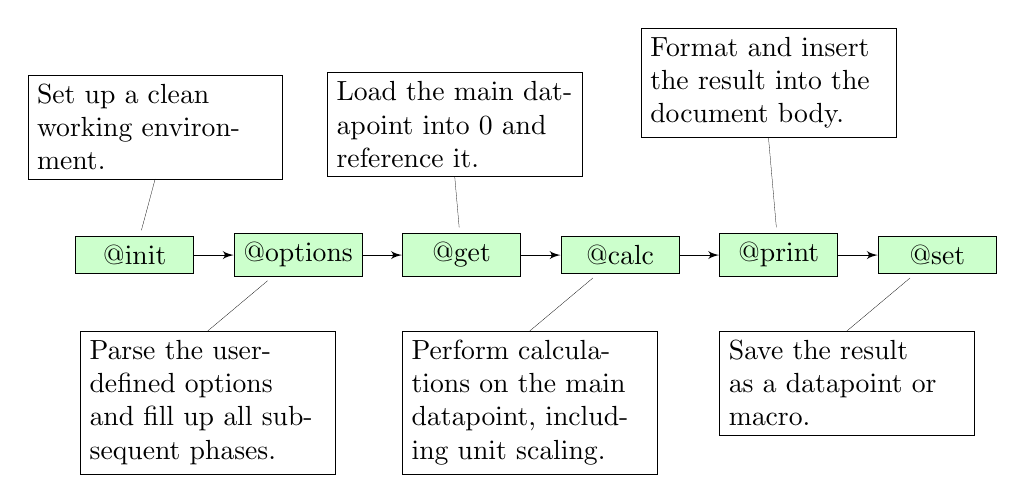
\begin{tikzpicture}[node distance=0.5cm]
    \tikzstyle{phase}=[draw,minimum width=1.5cm, fill=green!20!white];
    \tikzstyle{desc}=[align=left, text width=3cm,anchor=#1,draw];


   \node[phase](@init){@init};
   \node[phase,right=of @init](@options){@options};
   \node[phase,right=of @options](@get){@get};
   \node[phase,right=of @get](@calc){@calc};
   \node[phase,right=of @calc](@print){@print};
   \node[phase,right=of @print](@set){@set};

   \draw[>=latex']
     (@init) edge[->] (@options)
     (@options) edge[->] (@get)
     (@get) edge[->] (@calc)
     (@calc) edge[->] (@print)
     (@print) edge[->] (@set);

     \draw[ultra thin,shorten <=2pt] (@init) -- ++(75:1cm)
        node[desc=south] {Set up a clean working environment.};

      \draw[ultra thin,shorten <=2pt] (@options) -- ++(-140:1.5cm)
        node[desc=north] {Parse the user-defined options and fill up all subsequent phases.};

      \draw[ultra thin,shorten <=2pt] (@get) -- ++(95:1cm)
        node[desc=south] {Load the main datapoint into \cmd{\drefresult} and reference it.};

      \draw[ultra thin,shorten <=2pt] (@calc) -- ++(-140:1.5cm)
       node[desc=north] {Perform calculations on the main datapoint, including unit scaling.};

      \draw[ultra thin,shorten <=2pt] (@print) -- ++(95:1.5cm)
        node[desc=south] {Format and insert the result into the document body.};

      \draw[ultra thin,shorten <=2pt] (@set) -- ++(-140:1.5cm)
       node[desc=north] {Save the result as a datapoint or macro.};


     \end{tikzpicture}
     \caption{The \dataref Pipeline}\label{fig:pipeline}
   \end{figure}

   The \dataref macros are different regarding the phases they include or omit and in their default settings. In the
   following, we will discuss all options and macros you can use to reference your datapoints. By default, the
   \cmd{\drefresult} is always set to the result of the pipeline.

 \subsection{Setting Datapoints}



 \Macro[(@options, @set)]{\drefset\oarg{options}\{\meta{name}\}\{\meta{value}\}}


\begin{codeexample}
\begin{verbatim}
\drefset{/med A/mice race}{Black Six}
\drefset{/med A/mice count}{32}
\drefset{/med A/dead after 24h}{6}
\drefset{/med A/dead after 48h}{1}
\end{verbatim}
\end{codeexample}


 The \cmd{\drefset} command is used to define the symbolic datapoints. The name of a datapoint may contain virtually all
 characters, including spaces and slashes. It is good practice to use a hierarchy to structure your data point names.
 The value might be any string, while the focus of \dataref is on numerical datapoints. The \cmd{\drefset} command works
 outside the pipeline model (Figure \ref{fig:pipeline}) for performance reasons. It virtually consists only of the
 @options and @set stage.

 \Macro[(@options, @set)]{\drefsave[\meta{options}]\{\meta{name}\}\{\meta{value}\}}

 Besides setting the datapoint, \cmd{\drefsave} writes it to the \textsc{aux} file and, therefore, makes it available in
 the next \LaTeX{} run from the very beginning.

\subsection{Referencing Datapoints}


 \Macro[(@options=\{print=default\}, @get, @calc, @print, @set)]{\dref*[\meta{options}]\{\meta{name}\}}
 \Macro[(@options=\{print=raw\},     @get, @calc, @print, @set)]{\dref[\meta{options}]\{\meta{name}\}}

 This macro is used to reference a single symbolic data point. The value stored in that datapoint is inserted into the
 text. \cmd{\dref} additionally marks the data point as used; it will appear in the datagraphy (see
 Section~\ref{sec:datagraphy}). The starred variant does not attempt to parse the datapoint as a numerical value, but
 outputs the saved string.

\begin{example}
\dref*{/control group/mice race}\\
\dref*{/control group/mice count}\\
\dref[sci,precision=2,zerofill=true]{/med A/recovered}
\end{example}
\begin{codeexample}
\begin{verbatim}
\dref*{/control group/mice race}\\
\dref*{/control group/mice count}\\
\dref[sci,precision=2,zerofill=true]{/med A/recovered}
\end{verbatim}
\end{codeexample}

\Macro[(@get, @print)]{\drefvalueof\{\meta{name}\}}
\Macro[(@get)]{\drefref\{\meta{name}\}}
\vspace{1em}

\begin{example}
\drefvalueof{/med A/mice race}
\end{example}\begin{codeexample}
\begin{verbatim}
\drefvalueof{/med A/mice race}
\end{verbatim}
\end{codeexample}

  Since \cmd{\dref} is not expandable, it cannot be used in all circumstances. Therefore, \cmd{\drefvalueof} bypasses
  all internal bookkeeping and provides access to the raw datapoint value. \cmd{\drefref} can be used to mark the
  datapoint as used to let it appear in the datagraphy.

\Option[(default \textbf{true}, initially \textbf{false})]{/dref/ignoremissing=\meta{true-or-false}}
\Option[(no default, initially \textbf{1.0})]{/dref/defaultvalue=\meta{value}}

By default, \dataref produces an error if the referenced datapoint is undefined. If ignoremissing is given, the
defaultvalue is used. This key is useful in combination with \cmd{\drefsave}. Furthermore, it is possible to extract the
missing keys from the \textsc{aux} file and to retrieve it from a secondary source (e.g. database, wikidata, etc).

\begin{example}
\dref*[ignoremissing,defaultvalue=undefined]{blah}
\end{example}\begin{codeexample}
\begin{verbatim}
\dref*[ignoremissing,defaultvalue=undefined]{blah}
\end{verbatim}
\end{codeexample}

\Macro{\drefsethelp\{\meta{pattern}\}\{\meta{text}\}}
\Macro{\drefhelp\{\meta{name}\}}

 \textsf{dataref} comes with a simple method for defining documentation for data points. This help can for example be used to communicate what is the concrete semantics of the data point. This is of special interest when writter and data gatherer are not the same person. \cmd{\drefsethelp} takes two arguments: first a regular expression that matches the symbolic data point, second the help text.

\begin{codeexample}
\begin{verbatim}
\drefsethelp{.*/mice race}{The mice race used for experiments
 heavily influences the outcome of the results}
\end{verbatim}
\end{codeexample}

The documentation for a datapoint is obtained by using the \cmd{\drefhelp} macro. It checks all defined documentation
strings (in linear order, first defined, first matched), and prints the first matching help text. With \textbf{LuaTeX}:
only Lua (string.find) regular expressions are supported as patterns.

 \begin{example}
    \drefhelp{/med A/mice race}
  \end{example}\begin{codeexample}
\begin{verbatim}
\drefhelp{/med A/mice race}
\end{verbatim}
\end{codeexample}

\subsection{Calculations and Math Tools}

\Macro[(@options, @calc, @print, @set)]{\drefcalc[\meta{format}]\{\meta{expr}\}}
 \DescribeMacro{data("\meta{key}")}
 \DescribeMacro{d(\meta{key})}

 The \cmd{\drefcalc} command is the core function of calculating with data points. It is based on
 the pgfmath engine. It uses the required argument as a mathematical expression, but has additional
 features, that can be used.

 \begin{quote}
  \verb|\drefcalc{(4+7)/12 * 100}| $\Rightarrow$ \drefcalc{(4+7)/12 * 100}
 \end{quote}

 \noindent It adds support for the \texttt{data} function within pgfmath, which
 references symbolic data points. The keyname has to be in double
 quotes to indicate a string, but you can easily define an appropriate
 macro that abstracts from \verb|data("")|. As a quote-free
 alternative to the data command, \cmd{\drefcalc} provides also \verb|d(<key>|).



\begin{quote}
  \verb|\drefcalc{data("/med A/mice count") * 100}| $\Rightarrow$ \drefcalc{data("/med A/mice count") * 100}

  \verb|\drefcalc{d(/med A/mice count) * 100}| $\Rightarrow$ \drefcalc{d(/med A/mice count) * 100}
\end{quote}


 \noindent The optional argument lets you give a number format, which is used for printing the
 result number (\verb|/pgf/number format|).

 \begin{quote}
  \verb|\drefcalc[precision=5,fixed]{1/3}| $\Rightarrow$ \drefcalc[fixed,precision=5]{1/3}
 \end{quote}

 \cmd{\drefcalc} works always in a \textbf{/pgf/fpu} environment. The FPU feature of
 pgfmath is used to handle large numbers, which may occur often when handling experiment data
 points.

 \def\A{123456789}\def\B{987654321}\def\a{12}\def\b{98}

 \begin{tabular}{lrr}
 \multicolumn{3}{l}{\verb|\def\A{123456789}\def\B{987654321}\def\a{12}\def\b{98}|}       \\
 \toprule
 Macro                            & Inserted Text             & \cmd{\drefresult} \\\midrule
 \verb|\drefcalc{\A /\B}|  & \drefcalc{\A /\B}  & \drefcalc*{\A/\B}\drefresult       \\
 \verb|\drefcalc{\a /\b}|            & \drefcalc[]{\a /\b}          & \drefcalc*{\a/\b}\drefresult       \\
 \verb|\drefcalc*{\A/ \B}| & \drefcalc*{\A/\B} & \drefcalc*{\A /\B}\drefresult       \\
 \verb|\drefcalc*{\a /\b}|           & \drefcalc*{\a/ \b}         & \drefcalc*{\a /\b}\drefresult       \\
 \bottomrule
 \end{tabular}


 \DescribeMacro{\drefcalc*}
 \DescribeMacro{\drefresult}
 \DescribeMacro{\drefformat\{\meta{number}\}}

 \begin{quote}
  \verb|\drefcalc*{1/3} ABC: \drefresult| $\Rightarrow$ \drefcalc*{1/3} ABC: \drefresult\\
  \verb|\drefformat[fixed,precision=1]{\drefresult}|$\Rightarrow$ \drefformat[fixed,precision=1]{\drefresult}\\
  \verb|\drefformat[sci]{100000}| $\Rightarrow$ \drefformat[sci]{100000}
\end{quote}

\subsection{Units and Unit Scaling}

Datapoints can have a unit.

drefset'%
\drefset[unit=ms]{/duration B}{2}%
\drefset[unit=ms]{/duration}{5555}%
\drefset[unit=h]{/diff}{4}%
'

\drefkeys{
  unit/format default=siunitx,
  unit/new scala={1/y,365/d,24/h,60/m,60/s,1000/ms,1000/us,1000/ns},
  unit/new scala={1/\second,1000/\milli\second,1000/\micro\second,1000/\nano\second},
  unit/new scala={1/\kilo\joule,1000/\joule,1000/\milli\joule,1000/\micro\joule,1000/\nano\joule},
}


\foreach \a in {1234, 4135413, 213516513245, 24} {%
  \noindent\a
     $\rightarrow$ \drefformat[unit=\nano\joule,unit/scale to=\milli\joule]{\a}
     $\rightarrow$ \drefformat[unit=\nano\joule,unit/scale to auto]{\a}\\
}


dref,drefrel:'%
\dref[unit=\joule]{/duration};\drefrel[delta=/duration B]{/duration}'%

drefcalc:'%
\drefcalc[]{d(/duration) + 2}--after:\drefresult**\drefunit%
'

From save:'\drefcalc[ignoremissing]{d(/lateron)+d(/lateron 2)}'

drefcalc:'%
\drefcalc[scale by=2,unit/scale to auto]{d(/duration) + 2}--after:\drefresult**\drefunit%
'

\drefsave[unit=\milli\second]{/lateron}{3}
\drefsave[unit=\milli\second]{/lateron 2}{5}


\subsection{Relating Datapoints}

 \DescribeMacro{\drefrel*[\meta{opts}]\{\meta{key}\}}
 \DescribeMacro{\drefrel[\meta{opts}]\{\meta{key}\}}

 The \cmd{\drefrel} macro is used to calculate relations between
 different datapoints.. A prominent example of such a relation is the
 percent relation. \cmd{\drefrel} allows you to write down
 intentionally what relation you want to express without thinking
 about a concrete formula. The starred version of this macro does not
 print anything, but sets only \cmd{\drefresult}.

 \begin{quote}
 \noindent\verb|\drefrel[factor of=/med A/mice count]{/med A/recovered}| \\
 \mbox{}\hspace{1cm} $\Rightarrow$ \drefrel[factor of=/med A/mice count]{/med A/recovered} \\
 \end{quote}

 The type of relation is expressed with with various keys in a given
 order. The relation-key sequence performs calculations on the given
 data point. Like \cmd{\drefcalc}, \cmd{\drefrel} sets the
 \cmd{\drefresult} macro accordingly.

 \DescribeMacro{factor of=\meta{key or value}}
 \DescribeMacro{percent of=\meta{key or value}}

 Both relations are very similar, since they divide the current value
 by the given value. The \cmd{percent of} variant, scales the result
 by 100. The argument can be either a dataref key or a plain number.

 \[\cmd{\drefresult} = \frac{\texttt{value}}{\texttt{arg}}\]

 \noindent\verb|\drefrel[factor of=50]{/med A/mice count}| $\Rightarrow$ \drefrel[factor of=50]{/med A/mice count}\\
 \verb|\drefrel[percent of=/med A/mice count]{/med A/recovered}| $\Rightarrow$ \drefrel[percent of=/med A/mice count]{/med A/recovered}


 \DescribeMacro{increase by=\meta{key or val}}
 \DescribeMacro{overhead of=\meta{key or val}}

 It calculates the overhead factor towards the base value.
 \texttt{increase by} and \texttt{overhead of} are synonyms.

 \[\cmd{\drefresult} = \frac{\texttt{value} -
 \texttt{arg}}{\texttt{arg}}\]

 \verb|\drefrel[overhead of=50,fixed]{45}| $\Rightarrow$
 \drefrel[overhead of=50,fixed]{45}

 \DescribeMacro{delta=\meta{key or val}}

 Calculates the difference between value
 and base.

 \[\cmd{\drefresult} = \texttt{value} - \texttt{arg}\]

 \verb|\drefrel[delta=50]{45}| $\Rightarrow$
 \drefrel[delta=50]{45}

 \DescribeMacro{scale=\meta{key or val}}
 \DescribeMacro{product=\meta{key or val}}

It calculates the product of value and base.

 \[\cmd{\drefresult} = \texttt{value} \cdot \texttt{arg}\]

 \verb|\drefrel[scale by=2]{45}| $\Rightarrow$
 \drefrel[scale by=2]{45}

 \DescribeMacro{percent}

 Is a post-processing type. It calculates the percent value from a fraction.

 \[\cmd{\drefresult} = \cmd{\drefresult} \cdot 100.0 \]

 \noindent\verb|\drefrel[increase by=/control group/dead after 24h,percent]{/med A/dead after 24h}| \\
 \mbox{}\hspace{1cm}$\Rightarrow$ \drefrel[increase by=/control
 group/dead after 24h,percent]{/med A/dead after 24h}

\DescribeMacro{abs}

 Take the absolute value.

 \[\cmd{\drefresult} = \mid \cmd{\drefresult} \mid \]
 \verb|\drefrel[overhead of=50, abs]{45}| $\Rightarrow$
 \drefrel[overhead of=50, abs]{45}

  \DescribeMacro{negate}

 Is a post-processing type. It negates the value.

 \[\cmd{\drefresult} = \cmd{\drefresult} \cdot -1.0 \]

 \noindent\verb|\drefrel[factor of=/med A/mice count,negate]{/med A/recovered}| \\
 \mbox{}\hspace{1cm}$\Rightarrow$ \drefrel[factor of=/med A/mice count,negate]{/med A/recovered}

 \DescribeMacro{divide}
 \DescribeMacro{divide by}


 Divides the result by a factor.

 \[\cmd{\drefresult} = \cmd{\drefresult} \cdot \{divide\} \]

 \noindent\verb|\drefrel[divide by=1e6]{1453342654}|
 $\Rightarrow$
 \drefrel[divide by=1e6]{1453342654}

 \DescribeMacro{\drefprojection\{\meta{from}\}\{\meta{to}\}\{\meta{projection}\}}

 Sometimes one or multiple sets of data have to be projected/mixed into a
 new set of data that is fully dependent on those values. This is
 achieved with \cmd{\drefprojection}. It projects one data set (subdirectoy) into
 another one. Tithin the projection three different operations are
 possible: \cmd{\id}, \cmd{\rename} and \cmd{\calc}.

 \drefprojection{/control group}{/projection}{
       \id{mice race} % identity function
       \rename{mice count}{count} % renaming of points
       \calc{data("/dead after 48h")-data("/dead after 24h")}{died}
 }

 \begin{quote}
   \begin{verbatim}\drefprojection{/control group}{/projection}{
       \id{mice race} % identity function
       \rename{mice count}{count} % renaming of points
       \calc{data("/dead after 24h")-data("/dead after 48h")}{died}
     }\end{verbatim}

   \verb|\dref*{/projection/died}| $\Rightarrow$ \dref{/projection/died}\\
   \verb|\dref*{/projection/mice race}| $\Rightarrow$ \dref*{/projection/mice race}\\
   \verb|\dref{/projection/count}| $\Rightarrow$ \dref{/projection/count}
 \end{quote}

 \subsection{Various handy Tools}

 \DescribeMacro{\drefrow\{\meta{list}\}\{\meta{macro}\}}
 \DescribeMacro{\drefrow*}


 Often different columns in a table have to be obtained from your data
 points. Often those rows and columns are similar. Generating parts of
 tables within \LaTeX is very tricky, so \textsf{dataref} provides you
 with \cmd{\drefrow}. This macro iterates over a comma-separated list
 of values and fills out a macro which is interpreted as a symbolic
 data point. The entries are seperated with \& and printed. In the
 starred variant the resulting text is not interpreted as symbolic
 name, but as a macro. The symbolic name is expanded with \cmd{\drefvalueof}.

 The second argument is the macro, and can have two macro
 replacements. The first replacement \verb|#1| is the value of the list
 item, the second \verb|#2| is the index in the list.

 \begin{verbatim}\begin{tabular}{lccc}
   Group & $<$ 24h & $<$48h & recovered\\ \hline
   Control Group & \drefrow{dead after 24h,dead after 48h,recovered}%
                           {/control group/#1}\\
   Medicament A & \drefrow{dead after 24h,dead after 48h,recovered}%
                           {/med A/#1}\\
   Starred Variant & \drefrow*{B,C,D}{\#1=#1,\#2=#2}\\
 \end{tabular}
 \end{verbatim}


 \vspace{1em}\begin{tabular}{lccc}
   Group & $<$ 24h & $<$48h & recovered\\ \hline
   Control Group & \drefrow{dead after 24h,dead after 48h,recovered}%
                           {/control group/#1}\\
   Medicament A & \drefrow{dead after 24h,dead after 48h,recovered}%
                           {/med A/#1}\\\hline
   Starred Variant & \drefrow*{B,C,D}{\#1=#1,\#2=#2}\\
 \end{tabular}\vspace{1em}

 \DescribeMacro{\drefassert\{\meta{expr}\}}
 \DescribeMacro{[noassert]}

 Sometimes the underlying data changes while you are writing. But what
 if your prose text relies on certain characteristics of the data. \cmd{\drefassert} uses a pgfmath
 expression that evaluates to \verb|true| or \verb|false|. When the
 assertion holds (\verb|true|) nothing happens, only a terminal message
 is printed. When it does not hold (\verb|false|) the compilation is aborted.

 \begin{verbatim}\drefassert{data("/control group/mice count") > 30}
 Of the more than thirty infected mice...
 \end{verbatim}
 \drefassert{data("/control group/mice count") > 30}
 \begingroup \drefassert{data("/control group/mice
 count") > 30} \endgroup

 The \textbf{noassert} package options disables the latex abortion. In
 that case only a warning message is printed on the terminal.

 \DescribeMacro{[annotate=none]}
 \DescribeMacro{[annotate=footnote]}
 \DescribeMacro{[annotate=pdfcomment]}
 \DescribeMacro{[annotate=typeout]}


 While writing a document it is desirable to know, what key is used,
 while writing the text and generating the document. Therefore
 \textsf{dataref} provides the possibility to annotate values. The
 default package option \textbf{none} disables this kind of
 annotation. The \textbf{pdfcomment} option uses pdf
 annotations. Be aware that those annotations work properlyy only on a few
 selected PDF readers\footnote{In doubt use Acrobat}.

 \begin{quote}
   \verb|\drefkeys{annotate=none}|\drefkeys{annotate=none}\\
   \dref*{/control group/mice race}, \dref{/control group/mice count}, \drefcalc{100/3}
 \end{quote}

 \begin{quote}
   \verb|\drefkeys{annotate=footnote}|\drefkeys{annotate=footnote}\\
   \dref*{/control group/mice race}, \dref{/control group/mice count}, \drefcalc{100/3}
 \end{quote}

 \begin{quote}
   \verb|\drefkeys{annotate=pdfcomment}|\drefkeys{annotate=pdfcomment}\\
   \dref*{/control group/mice race}, \dref{/control group/mice count}, \drefcalc{100/3}
 \end{quote}

 \subsection{Datagraphy}\label{sec:datagraphy}

 \DescribeMacro{\drefusagereport}
 \DescribeMacro{[usagereport]}
 \DescribeMacro{[refall]}

 With the \textbf{usagereport} package option enabled,
 \cmd{\drefusagereport} generates a usagereport of all referenced
 keys. The usage report groups the keys by the help texts. If the
 refall package option is given, all keys are marked as referenced.

 \section*{Datagraphy}
 \drefusagereport

\end{document}

%%% Local Variables:
%%% mode: latex
%%% TeX-master: t
%%% End:
